% =============================================================================
%  Sección 2: La Metamorfosis del Territorio: Cambios por Crecimiento Urbano
% =============================================================================

\section{La Metamorfosis del Territorio: Cambios por Crecimiento Urbano}

En esta sección abordaremos los cambios urbanos a tres niveles: El avance de una metropoli que no para de crecer, 
la constante población que debe atender sus necesidades en un territorio que el gobierno ha decidido ignorar y finalmente
los estragos de una periferia relegada a su suerte o con falta de planeación y planificación. En este caso, abordaremos el 
tema bajo dos perspectivas claras: Mientras el norte se desarrolló un proyecto de humedales en Sna Juan de Aragón para la 
preservación ecológica del mismo, en el centro-sur se le relegó a los humedales a zonas de contaminación y exclusión social.

\subsection{El avance de la mancha urbana}

La expansión urbana en el SC, aunque legalmente prohibida, ha proliferado de manera centrífuga y fragmentada \cite{rojas2020deterioro}.
Históricamente, la desecación de los lagos y la pavimentación han alterado la recarga de los acuíferos. En la zona lacustre de Xochimilco, 
la mancha urbana se ha intensificado en las últimas tres décadas, duplicando el número de viviendas en barrios críticos como San Francisco Caltongo 
entre 2005 y 2010 \cite{rojas2020deterioro}. Como se observa en la cartografía de la zona (ver Figura \ref{fig:asentamientos_mapa}), los límites del 
área protegida son vulnerados constantemente por la dinámica inmobiliaria informal.

\begin{figure}[ht]
    \centering
    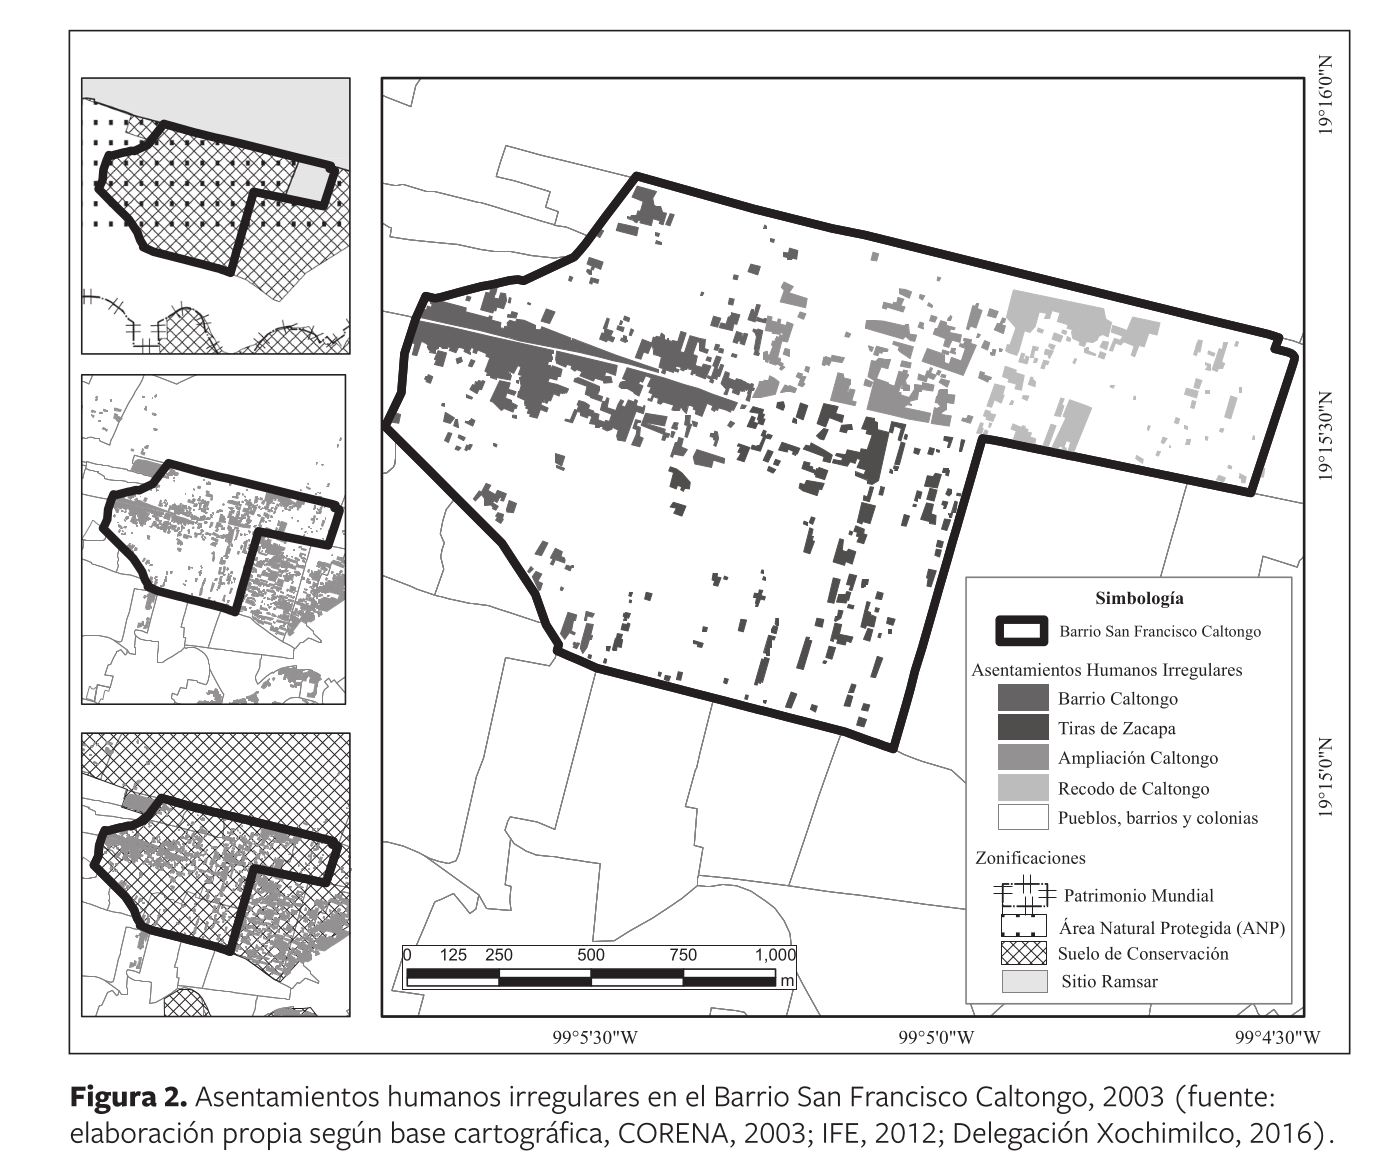
\includegraphics[width=0.8\textwidth]{img/Fig2_Asentamientos_Humanos_irregulares.png}
    \caption{Asentamientos humanos irregulares en el Barrio San Francisco Caltongo y su interacción con las zonas de protección.}
    \label{fig:asentamientos_mapa}
\end{figure}

\subsection{Asentamientos irregulares}

La falta de acceso a vivienda asequible ha forzado a los sectores más pobres a ocupar zonas no aptas para la urbanización. 
En el caso de San Francisco Caltongo, se identifican cuatro asentamientos principales: Ampliación Caltongo, Barrio Caltongo, 
Tiras de Zacapa y Recodo de Caltongo \cite{rojas2020deterioro}. La densidad de población en estos sitios es alarmante; la Figura 
\ref{fig:habitantes_grafico} detalla el número de habitantes por asentamiento, destacando Ampliación Caltongo como el núcleo de mayor presión demográfica.

\begin{figure}[ht]
    \centering
    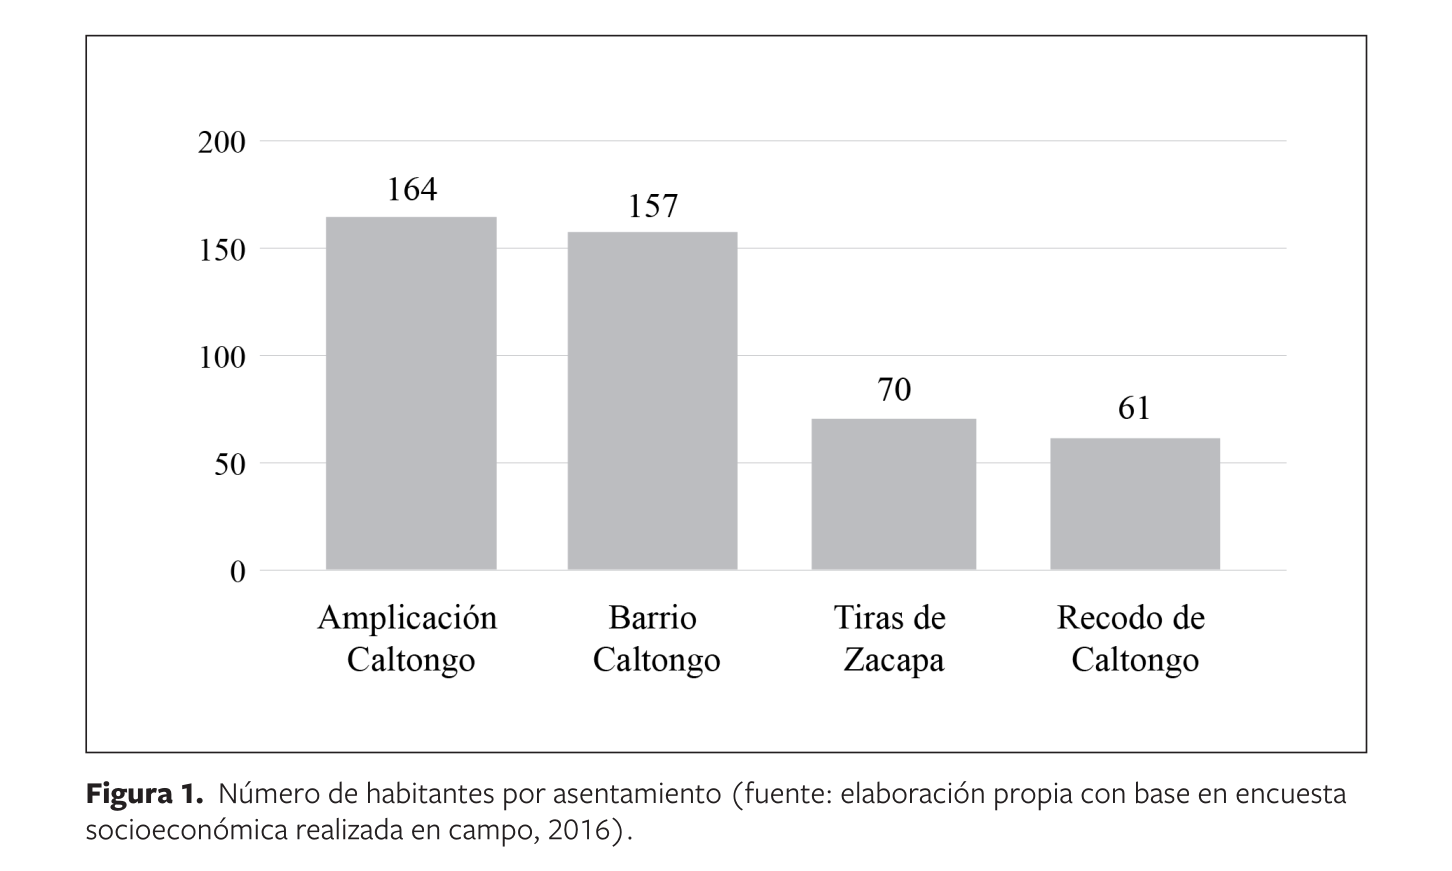
\includegraphics[width=0.7\textwidth]{img/Fig1_Numero_habtiantes_asentamientos.png}
    \caption{Número de habitantes por asentamiento irregular en la zona lacustre.}
    \label{fig:habitantes_grafico}
\end{figure}

Esta ocupación irregular conlleva consecuencias ecológicas directas: al carecer de red de drenaje, los residentes recurren a la autogestión informal. 
En Xochimilco, se estima que existen más de 1,300 descargas de aguas residuales (grises y negras) vertidas directamente a los canales \cite{rojas2020deterioro}. 
Caltongo destaca como el barrio con el mayor índice de contaminación por estas descargas, según se ilustra en la Figura \ref{fig:descargas_barrios}.

\begin{figure}[ht]
    \centering
    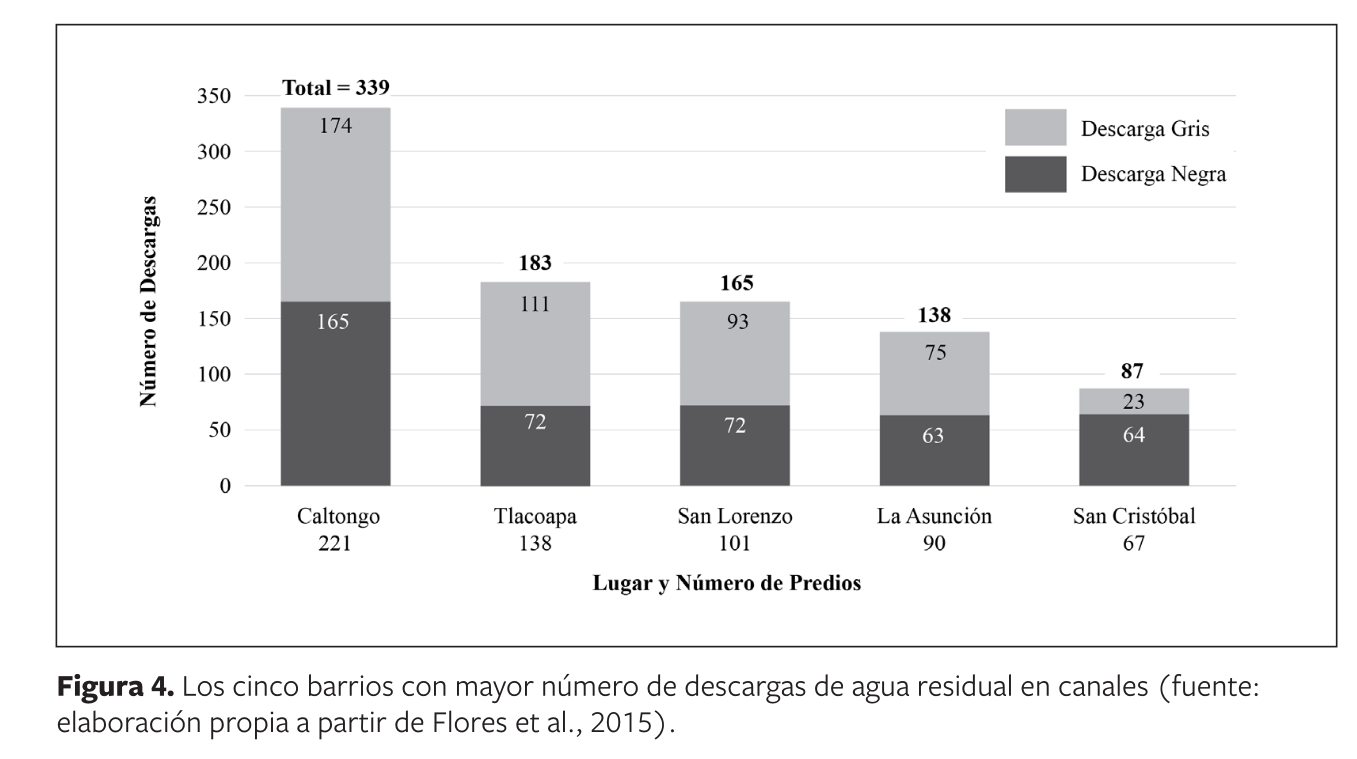
\includegraphics[width=0.7\textwidth]{img/Fig4_Barrios_descarga.png}
    \caption{Barrios con mayor número de descargas de agua residual en los canales de Xochimilco.}
    \label{fig:descargas_barrios}
\end{figure}

\subsection{Construcciones y deforestación}

La fragmentación del hábitat es el resultado más severo de la infraestructura vial y habitacional. La compactación del suelo por la construcción de viviendas informales,
muchas veces utilizando materiales precarios o cascajo para rellenar canales, reduce drásticamente la permeabilidad del territorio \cite{rojas2020deterioro}. 
Este proceso se ve agravado por la sustitución de vegetación nativa por especies introducidas y la tala para despejar cables de energía eléctrica instalados ilegalmente, 
lo que aumenta el riesgo de incendios y la pérdida de biodiversidad endémica \cite{rojas2020deterioro}. A diferencia del modelo de Aragón, donde se busca la regeneración 
de la cubierta vegetal, en Xochimilco el avance urbano está íntimamente ligado a la degradación irreversible del paisaje natural.
